 \item Modyfikacja danych części - scenariusz główny \\
 
 Opis słowny - ten przypadek użycia opisuje funkcjonalność modyfikacji danych istniejących typów części. Obejmuje to sytuację, gdy np. cena danej części musi zostać zmieniona.
 
 \begin{longtable}{|p{5cm}|p{7cm}|}
 	\hline
	\textbf{Aktor} & Pracownik \\
	\hline
	\textbf{Warunki początkowe} & Posiadanie konta z uprawnieniami umożliwiającymi zarządzanie częściami, zalogowanie się do systemu \\
	\hline
	\textbf{Opis przebiegu interakcji} & Wybór prezentacji listy części na stronie głównej sklepu, wybranie opcji modyfikacji konkretnej części, wprowadzenie danych, zatwierdzenie operacji \\
	\hline
	\textbf{Sytuacje wyjątkowe} & Podanie błędnych danych przy modyfikacji części \\
	\hline
	\textbf{Warunki końcowe} & Modyfikacja danych wybranej części \\
	\hline
 \end{longtable}
 
  \item Modyfikacja danych części - scenariusz główny \\
  \begin{tabularx}{\linewidth}{ c X}
  Aktor: & Pracownik \\
  \end{tabularx}
   \begin{enumerate}
    \item Scenariusz ``Wyświetlanie listy części - scenariusz alternatywny - użytkownik posiada specjalne uprawnienia do zarządzania częściami''. \label{modyfikacja-czesci-poczatek}
    \item Pracownik wyszukuje na liście część którą chce zmodyfikować i wybiera przycisk modyfikacji.
    \item System prezentuje pracownikowi formatkę taką jak dla dodania nowej części, ale wypełnioną danymi modyfikowanej części, z możliwością ich edycji. Dodatkowo, istnieje możliwość edycji liczby części wybranego typu, znajdujących się aktualnie w magazynie.
    \item Pracownik modyfikuje wybrane pola i zatwierdza operację. \label{modyfikacja-czesci-zatwierdzenie}
    \item System modyfikuje część w bazie danych i informuje użytkownika o zakończeniu operacji.
  \end{enumerate}
  
  \item Modyfikacja danych części - scenariusz alternatywny - podanie błędnych danych przy modyfikacji części \\
  \begin{tabularx}{\linewidth}{ c X}
  Aktor: & Pracownik \\
  \end{tabularx}
   \begin{enumerate}
    \item Kroki \ref{modyfikacja-czesci-poczatek} do \ref{modyfikacja-czesci-zatwierdzenie} scenariusza głównego.
    \item System sprawdza czy zmodyfikowane przez użytkownika dane są poprawne, czyli:
    \begin{enumerate}
      \item Czy wszystkie pola oprócz opisu i zdjęcia są wypełnione
      \item Czy podana cena nie jest ujemna
      \item Czy podana minimalna liczba sztuk na magazynie nie jest ujemna
      \item Czy podana aktualna liczba sztuk na magazynie nie jest ujemna
    \end{enumerate}
    \item W przypadku niepoprawności wprowadzonych danych, system wyświetla stosowny komunikat błędu i anuluje operację. W przeciwnym przypadku powrót do scenariusza głównego.
  \end{enumerate}
  	
\begin{figure}[h!]
    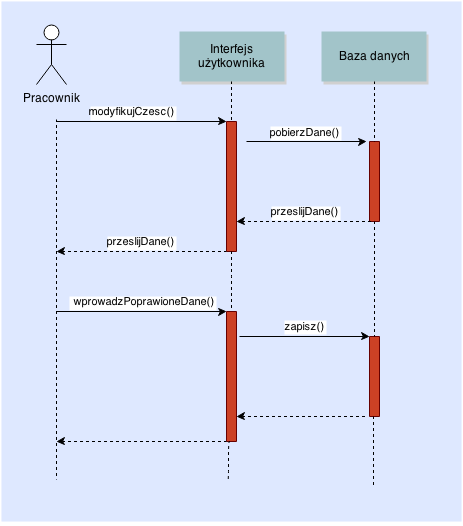
\includegraphics[width=\textwidth,
    height=0.7\textheight]{graphics/UseCase/Czesci/ModyfikacjaCzesciSD.png}
  \caption{Diagram sekwencji dla przypadku użycia Modyfikacja części - scenariusz główny}
\end{figure}